
\section{Workload management\label{sec:Queuing}}

\subsection{Overview\label{sec:OverviewQueuing}}

We cover here the different aspects of the management of heterogeneous workloads involving quantum and high-performance classical resources. Whereas both technologies have an extensive set of functional tools for resource access and management, scheduling, and data handling, there is still need for substantial work towards extending the elasticity of these tools to operate in a hybrid quantum-classical environment and to cater for the needs of the different user profiles. 

We consider and discuss the specificities of different access models, with classical and quantum resources operating in co-located environments or remotely, and explore the impact that different integration timescales, given the disparity in speed and bandwidth between quantum and classical, have on such operational models.

Finally, we describe the current state of the middleware layer for quantum and classical integrations across many different vendors in the industry and give some brief overview of their challenges and involved complexities.


Computational workloads can be categorized broadly into two classes:
(1) trivial (or ``embarrassingly parallel'') tasks, where each task executes independently of all others using its own set of dedicated computational resources;
and (2) non-trivial interoperating sets of tasks, potentially sharing an allocated set of computational resources, where the outcome of a subset of tasks can affect the behavior of another. For HPC systems to handle the various requirements of such workloads, sophisticated workload management systems (WMS) and job schedulers enable efficient resource allocation, initiate and monitor workload execution, and govern a queue of pending work requesting resources.

In quantum-centric supercomputing systems, computational workloads can also be defined based on Quantum-HPC integration types, such as HPC-for-Quantum, Quantum-about-HPC, Quantum-in-HPC scenarios, involving interplay between quantum and classical tasks. Consistency in Quantum-x-HPC or HPC-x-Quantum seems desirable and possible. Quantum-about-HPC workload involves quantum tasks that require HPC resources for pre- and post-processing. In this integration type, the quantum tasks are independent of the HPC tasks, and the HPC resources are used to support the quantum tasks. Quantum-in-HPC workload involves HPC tasks that require quantum resources for acceleration, where the quantum tasks are tightly coupled with the HPC tasks, and the HPC resources are used to support the quantum tasks. 


Finally, HPC-for-Quantum workload involves tight integration with quantum resources in real-time, within the coherence time of the quantum system \ref{realtimeQuantumClassical}. The classical resources are used to support the quantum tasks, and the classical tasks are tightly coupled with the quantum tasks~\cite{saurabh2023conceptual}. Circuits with classical control often referred as \textit{dynamic circuits}.

As discussed above, integrating quantum systems into classical HPC facilities will add complexity to managing and scheduling quantum-based workloads due to the disparity between quantum and classical processing times, sometimes requiring dynamically allocating and deallocating resources within and among jobs.

In this section, we discuss in detail challenges related to classical-quantum workload management, job scheduling, queuing, and operation modes of these jobs.
We review these concepts and current solutions in the classical setting, and give recommendations for
on-premises and cloud-based integration of quantum computational resources with HPC systems.


We differentiate between (i) on-premises integration, which involves directly incorporating quantum computational resources within a local HPC system infrastructure, and (ii) cloud-based integration, which entails accessing quantum computational resources remotely through cloud services.
Scenario (i) suits workloads requiring tight integration between quantum and classical resources (e.g., Quantum-in-HPC and HPC-for-Quantum workloads). Further, it is ideal for sensitive or proprietary workloads where data security and privacy are paramount, as the data does not leave the premises. Scenario (ii) is beneficial for workloads that can tolerate latency, e.g., Quantum-about-HPC workflows that offload encapsulated parts to a cloud quantum system.




\subsection{Resource management}

This section is structured into two main parts: exploring the resource model, which deals with the allocation and architecture of quantum computing resources, and job scheduling, which is essential for optimizing the performance and efficiency of quantum computing tasks.

\subsubsection{Resource model}

A resource model refers to the framework or method used to manage and allocate computational resources. Specifically, in this section, we explore the distinction and relationship between Quantum Processing Units (QPUs) and qubits, the placement and location of quantum and classical resources and ownership models.


\paragraph{\textbf{QPU vs qubits}}

The introduction of quantum processing units (QPUs) marks a significant departure from the conventional approach to traditional high-performance computing (HPC) scaling. Instead of pursuing the conventional path of continually improving semiconductor processors for greater speed and density, or incorporating specialized processors like GPUs, and optimizing their coordinated use through parallelization, QPUs take a fundamentally different approach. While one might assume that QPUs merely serve as an additional component, they fundamentally alter the way data is represented, employing the language of quantum circuits governed by the principles of quantum mechanics. This constitutes a distinct computational model, diverging from all that has come before it. However, it's essential to note that QPUs are not designed for general-purpose computing tasks. Consequently, practical implementations necessitate the careful orchestration of both classical and quantum computation resources.

Of particular importance for this type of scheduling task is the fact that QPUs operate at very different time scales and bandwidths from standard HPC processes. One could argue that the quantum circuit represents the essence of QPUs as co-computing units with very specific tasks in a supercomputing environment. As the fundamental unit of quantum information, the quantum circuit is a computational routine consisting of coherent quantum operations, including unitary transformations and projective measurements, and concurrent classical computation. As such computational units, quantum circuits may require executions that span inordinate amounts of time for a single computation. For example, consider the fastest quantum hardware that exists today at scale, superconducting qubits, tackling the task of running a circuit with 100 qubits and $10^8$ $T$ gates. Using the surface code, and assuming a physical error rate of $10^{-4}$ and a syndrome cycle time of 1 $\mu$s, a single execution of that circuit, considering both magic state distillation and consumption, can take on the order of tens of minutes and up to several hours, depending on the number of state distillation factories (and therefore physical qubits) used~\cite{litinski2019game}. This circuit execution cannot be preempted, which is important for scheduling purposes. 

The above scenario represents an ideal, still far from what quantum hardware can offer today. Currently, QPUs don’t run in fault tolerant ways, can only tackle much smaller circuits, and must leverage error mitigation solutions that result in large sampling overheads. In contrast with the example above, QPUs today are extremely non-fungible, each of them with its own noise profile, and this affects user preferences and scheduling complexity. 

The introduction of this new type of resource opens a range of models of operation:

\textit{QPU-based Model}: This model resembles the current GPU model, where the entire quantum device is treated as a unified resource unit. Due to its natural inflexibility, this approach has the downside of potential device underuse when jobs only target a subset of the QPU.

\textit{Qubit-Based Model}: In this approach, the qubits themselves are treated as resources, allowing a QPU to be fully occupied simultaneously by a variety of jobs. In near-term devices, with qubits exhibiting different types and amount of noise, and in the presence of limited device connectivity, this approach has shortcomings, as there would be competition among jobs for the best or more suited resources within the QPU.

\textit{Shares Model}: This introduces a pseudo-unit of resource definition where each ``share'' represents a part of the device, a specific period of time, or the circuit size. Essentially, each share signifies a portion of the computational capacity of the resource. Can be treated as sub-category or QPU-based model \cite{qiskitRuntimeFairShareAdmin}.




\paragraph{\textbf{Quantum resource location.}}

In the landscape of HPC, the location of computing resources determines the efficiency, performance, and accessibility of computational tasks. Two primary modes of resource location, co-located and remote resources, offer distinct advantages and considerations for HPC facilities and users.



\textit{Co-located resources} refer to computational resources physically situated within the same facility or data center as the user or workload management system. There are several advantages of having co-located quantum and classical resources. Minimal network latency and high-speed data transfer capabilities, which is especially advantageous for applications where access to large amounts of (low-level) data (like counts) is required. Full control and management of co-located resources, enabling customization and configuration based on specific requirements. Data security. Co-located resources location implements on-premises integration type (i) \ref{sec:OverviewQueuing}.

\textit{Remote quantum resources}, on the other hand, are located at a physical distance from HPC classical infrastructure, often in off-site data centers, cloud environments (cloud model integration type (ii) \ref{sec:OverviewQueuing}), or partner organizations. Remote resources extend the reach and capabilities of HPC systems, but they come with unique characteristics. Elasticity is one of them, allowing for scaling up and down quantum resources based on need. Another characteristic is sharing. At this moment, it is a case when a quantum processor is shared among multiple users, which drives down the cost of execution, but also introduces variation in performance due to resource contention. Network overhead can impact data transfer rates and communication latency, especially in applications with large loads. 

\paragraph{\textbf{Quantum resource ownership.}} 
\label{sec:WM_ResourceOwnership}


High-performance computing facilities generally serve large numbers of users with varying computational resource requirements for their computational workloads (jobs) \ref{sec:DataPreprocessing}.
Users are part of user groups and projects, which have assigned queues.
A project has some resource allocation quota (e.g., $10^{6}$ node hours), whereas queues are defined by criteria such as priority and the amount of computational resources available per job (e.g., $n$ CPU cores, $m$ GPUs) to a user of that queue.
At the level of user groups and projects, the integration of quantum information processing devices with classical HPC computational resources is straightforward: access to a quantum resource could be granted to a given user assigned to a \texttt{qpu\_user} group with project quota $Q$ specifying the number of ``quantum node'' hours.



\begin{figure*}
    \centering
     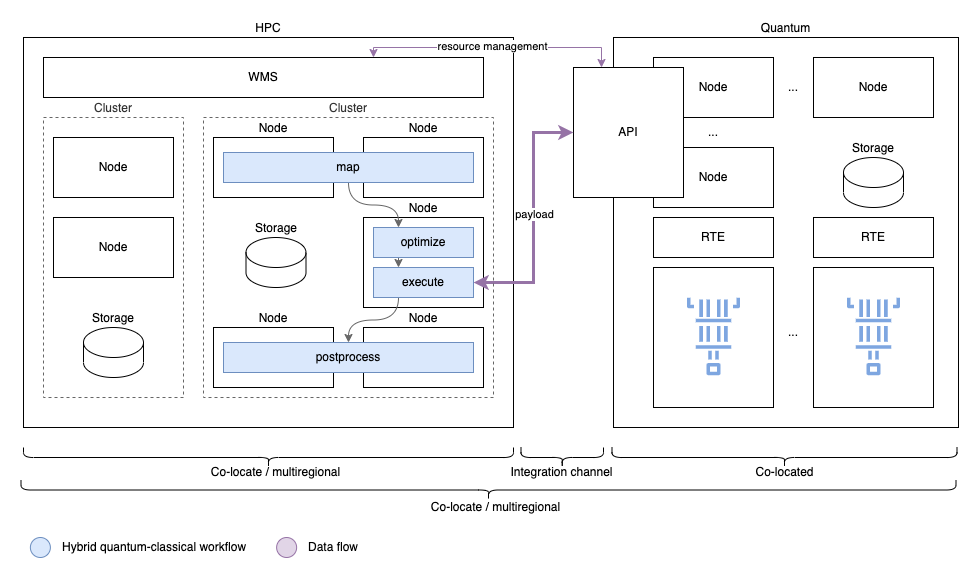
\includegraphics[width=0.85\textwidth]{groups/4._Queueing/images/hpc-quantum-integration.png}
    \caption{Quantum-centric supercomputing integration overview. Integration channel can be tight or loosely coupled, which will affect throughput and latency of transmitted payload. Real-time compute is possible on co-located quantum side; near-time compute can be executed on quantum and HPC sides; long-time compute should happen on HPC side. Depending on implementation WMS can schedule tasks on quantum side through API or direct access to classical nodes of quantum side.}

    
    \label{figure:HPCQuantumIntegration}
\end{figure*}

\begin{figure}
    \centering
     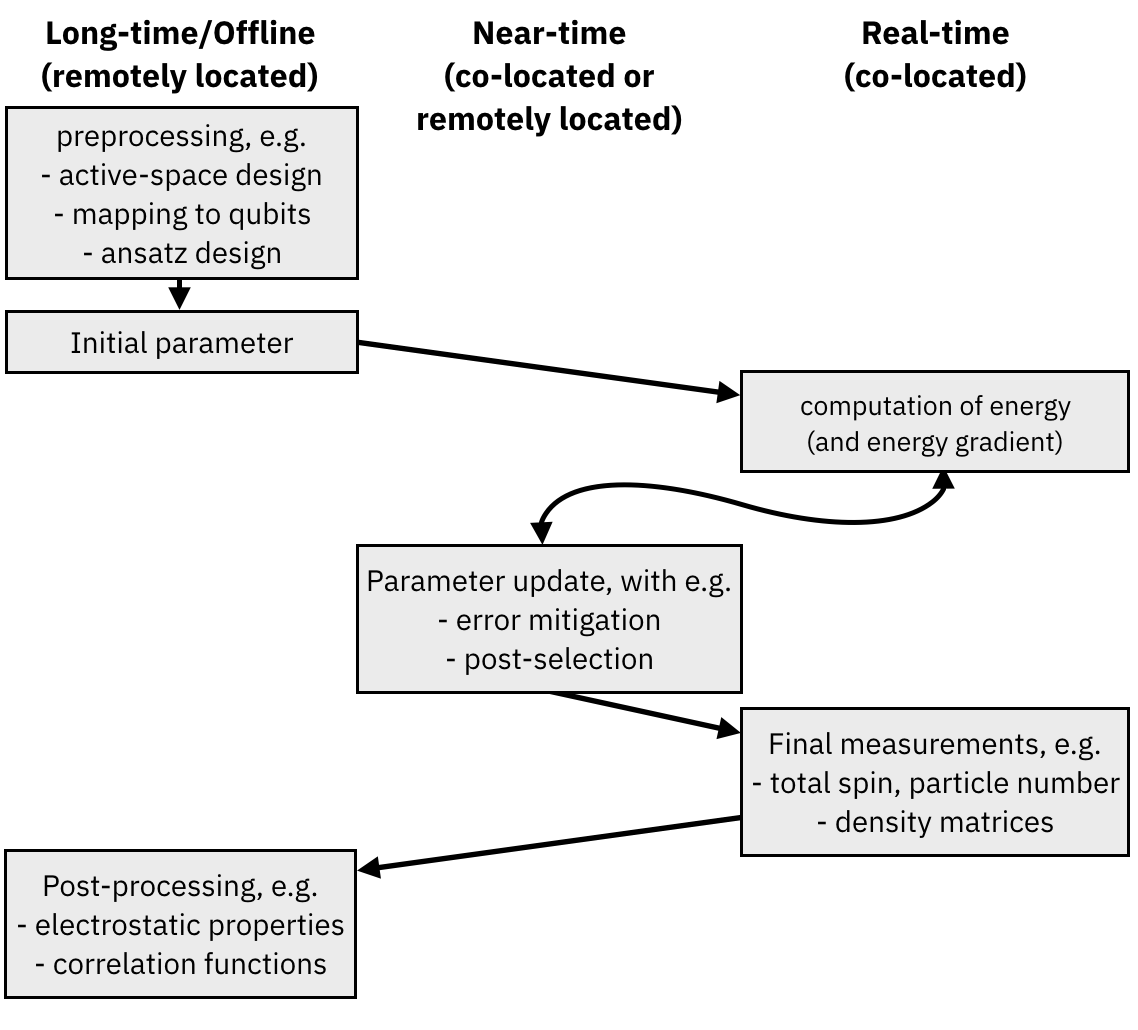
\includegraphics[width=\columnwidth]{groups/4._Queueing/images/example_integration.png}
    \caption{Integration between classical (HPC) and quantum computing resources exemplified by the variational quantum eigensolver. The steps of the calculation are represented by gray blocks, connected by arrows describing the flow of operations and arranged left/center/right for operation that require ``long-time/near-time/real-time'' interaction between HPC and quantum computers (see also main text). 
    }
    \label{figure:HPCQuantumIntegrationExample}
\end{figure}



\subsubsection{Job Scheduling}

When introducing quantum resources, one could envisage \textit{real-time} quantum nodes, where classical computations are performed within the coherence time of the qubits (e.g., for error correction studies), and \textit{near-time} quantum nodes, where higher latency classical communication suffices (e.g., variational algorithms).

Common frameworks in use today within HPC facilities and cloud platforms include SLURM~\cite{yoo2003slurm}, TORQUE~\cite{torqueengine}, Altair Grid Engine~\cite{altairgridengine}, and IBM Platform LSF~\cite{ibmlsf}, which provide highly scalable control over heterogeneous computer clusters and jobs submitted to them.
To execute a workload, a user configures their job using a \textit{submission script} based on the syntax of the associated scheduler.
Submission scripts essentially define a job:
project name, resource requirements (e.g., node count, CPU count, memory size, and wall clock limit), tasks to execute, input and output data paths, etc.
Note the governance of an HPC system (see Sec.~\ref{sec:queuing:gov}) could require all input data be readily available, e.g., on a scratch area accessible only by the user.
These scripts are submitted from a login (head) node to the WMS or job scheduler, where they are queued and finally executed on one or more compute nodes.

A queued user job is executed in the order of the project's or queue's priority as well as resource availability;
for instance, a higher-priority job whose resource requirements are met will be executed before a lower-priority job.
Resources can be exclusive or shared, so if \texttt{job\_x} does not need all cores on the node(s) to which it is assigned, \texttt{job\_y} could be assigned to the remaining cores.
However, resources allocated to a given job are fixed and, therefore, remain allocated for the duration
of the job's lifetime (and thus charging against the user/project quota), regardless of whether or not they are performing useful work.


Extensions to existing job schedulers could include quantum-specific configuration settings, e.g.,
number of circuits to be executed and depths, from which, along with architecture-dependent factors such as data loading, gate application, and readout times, runtime estimates can be made.
However, while separating classical and quantum configuration spaces may be amenable to near-term
applications (i.e., wherein classical and quantum operate cooperatively but have loose latency requirements, as in VQE),
mid-term quantum-classical applications requiring lower latencies likely will necessitate tighter integration between the two types of resources.



Additionally, quantum-centric supercomputing workload scheduling must also consider the coupling between the quantum and classical tasks and assign and co-locate tasks to the resources accordingly. Different quantum-classical coupling types represent workloads with unique requirements and challenges, such as the lack of a unified standard for accessing QPUs and expressing hybrid workloads, and the need for parallelization of quantum workloads across nodes, cores, and accelerators. For example, classical tasks tightly coupled to quantum tasks, e.g., for the HPC-for-Quantum integration type, must be co-allocated and assigned to nearby QPUs and GPUs. Additionally, scheduling of  QPU jobs must be prioritized to ensure the optimal utilization of the QPUs while minimizing the time-to-solution and energy-to-solution~\cite{saurabh2023conceptual} (section \ref{queueing}).


\paragraph{\textbf{Queueing}}
\label{queueing}

HPC environments typically offer shared resources that are made available to a large user base. To ensure the equitable and efficient distribution of computing resources, HPC systems implement queuing mechanisms. 

One of the aspects of execution management in HPC is the presence of multiple queues, each configured with specific priorities and constraints. These queues are designed to categorize and prioritize computational tasks based on the specific needs and requirements of the users or projects.

Queues can have resource constraints. Resource constraints may include limitations on the number of nodes, processors, memory, or specific software specifications available for jobs in each queue. These constraints help balance the allocation of resources across different user groups and projects while ensuring that the computing environment remains stable and efficient.  As QPUs are "rare" resources, it is beneficial to increase the priority of the "quantum" queue while maintaining constraints on execution time and classical resources. It might be also beneficial to increase the priority of classical jobs connected to the quantum queue.

Because QPUs are a new and currently limited resource type, it is beneficial to specify a separate queue for quantum jobs.

Furthermore, as quantum computing technology evolves and the number of available QPUs increases, HPC administrators will need to adapt the queuing system to accommodate this growth. This might involve not only adjusting the priority of the quantum queue but also dynamically redistributing workloads to make optimal use of the expanding quantum infrastructure. Balancing the allocation of quantum and classical resources will remain a complex task, requiring constant monitoring and fine-tuning to ensure efficient utilization of the entire HPC facility. In this context, the queuing system's flexibility and adaptability will be crucial in meeting the evolving demands of quantum computing within the HPC environment.

\textit{Cloud queues}. There is a practice nowadays of cloud vendors are providing access to quantum services that are executing quantum payload. In order to provide fair allocation of resources, cloud providers are implementing their own queuing mechanisms behind cloud endpoints. It is important to understand that cloud vendors have different job queuing and priority implementations, and all might employ a shared resource ownership model \ref{sec:WM_ResourceOwnership}. 

\textit{Qiskit Runtime service fair share queue}. Access to quantum resources are divided between hubs, groups and projects.
A \textit{Hub} represents the top level of an organization such as an academic, industry, or research partner.
A \textit{Group} represents a mid-level structure to which access shares can be allocated by the hub for one or more collections of users (projects).
A \textit{Project} represents the base-level construct to which shares are allocated from the overarching group, and to which users are directly assigned.

For each group and project, the duration of the scheduling period is used to convert shares into an equivalent amount of time that an instance would receive under ideal conditions. The ratio between the time used and the shares equivalent time is used as the basis for scheduling jobs.

Many HPC job scheduling systems employ a so-called "fair-share algorithm" designed to distribute computational resources among multiple jobs in a manner that is considered fair. The definition of "fair" can vary significantly depending on the context and the specific requirements of the system. The Qiskit Runtime fair-share algorithm takes into consideration how shares of resources are distributed across groups and projects to determine job prioritization \cite{qiskitRuntimeFairShare}.


\paragraph{\textbf{Cloud-bursting model}}



Similar to a classical cloud bursting \cite{bicer2011cloudbursting}, we propose a Quantum cloud bursting model in which an HPC facility offloads quantum computation to cloud vendors when there are insufficient quantum resources within its local infrastructure.

As with any approach, there are pros and cons of quantum cloud bursting. 
Quantum resources may be expensive to maintain locally. In such cases, offloading workloads to cloud vendors with readily available QPUs can significantly decrease maintenance. 
Certain applications require proprietary or specialized software. Acquiring and managing licenses for such software can be both costly and time-consuming. Cloud bursting allows organizations to leverage cloud vendors' pre-configured environments, providing access to the required software without local setup and licensing.
It also presents challenges related to data transfer and increased requirements for security.


\begin{table*}[t]
    \centering
    \begin{tabularx}{\textwidth}{@{}>{\bfseries}l*{3}{X}@{}}
        \toprule
        Endpoint & Request Body & Response & Description \\
        \cmidrule(r){1-4}
        \it{GET allocations/} 
            & \makecell[l]{allocation\_ids: list(str) \\  fields: list(str)}
            & allocations: list(dict)
            & Fetch resource allocations listed by id. \\
        \it{POST allocations/} 
            & specification: dict
            & allocation\_id: str
            & This allocates a set of resources from a resource request specification. \\
        \it{DEL allocations/} 
            & allocation\_id: str     
            & status: bool
            & Destroy a resource allocation and return resources to the pool of available resources. \\
        \it{GET resources/} 
            & \makecell[l]{specification: dict \\  fields: list(str)}   
            &  resources: list(dict)
            & Fetch the current state of resources on a system.  This should report status of anything that a user may be able to specify for their job placement, including QPU status and software stack status \\
        \it{GET tasks/} 
            & \makecell[l]{task\_ids: list(str) \\  fields: list(str)}
            & tasks: list(dict)
            & If a list of tasks are passed in, provide information on currently running tasks on the system.  If no tasks passed in, provide information on all running tasks.  This may constrain the results for the executing user so that it shows only their own jobs if the user is otherwise unprivileged. \\
        \it{POST tasks/} 
            & \makecell[l]{task\_information: dict \\  allocation\_id: str \\ batch\_id: str}  
            & allocation\_id: str
            & Launch a task. \\
        \it{DEL tasks/} 
            & \makecell[l]{task\_ids: list(str) \\  signal: int} 
            & status: bool
            & Send a signal to tasks for termination. \\
        \bottomrule
    \end{tabularx}
    \caption{Minimal quantum cloud bursting API specification.}
    \label{table:quantum_cloud_bursting}
\end{table*}


Figure \ref{figure:HPCQuantumIntegration} is showing how quantum cloud bursting model can be implemented via integration of Quantum cloud API and workload management system. Table \ref{table:quantum_cloud_bursting} shows a minimal API specification that cloud vendors should implement to unlock better integration of quantum and classical resources.

An illustration is given in Figure \ref{figure:HPCQuantumIntegrationExample}, using the variational quantum eigensolver as an example. Classical preprocessing (including mapping to qubits, choice of the variational ansatz, and parameter initialization) is carried out on HPC resources located remotely from the quantum computer (``long-time'' interaction). The execution of quantum circuits may require the use of real-time communication between classical and quantum units through real-time electronics of RTE (see also Figure \ref{figure:HPCQuantumIntegration}). Real-time interaction is required e.g. to implement dynamical circuits used for symmetry verification/enforcing, monitored quantum dynamics, and quantum error correction.
The update of variational parameters, which requires the calculation of energies and energy gradients typically in conjunction with readout/gate error mitigation and post-selection operations, may be carried out on HPC resources located remotely from the quantum computer or co-located with it (``near-time'' interaction).

\paragraph{Quantum execution runtime prediction}

Quantum execution runtime, determined by circuit complexity (number and type of gates, layers), can be predicted using historical data~\cite{ravi2022adaptive}. Despite potential overhead from error mitigation and circuit transpilation, accurate predictions are achievable. However, dynamic circuits with their non-deterministic workload structures pose challenges. 

Runtime prediction is crucial for effective workload management, allowing quantum resources to be optimally utilized. Incorporating runtime predictions into scheduling enhances priorities and overall workload efficiency, showcasing the valuable role of prediction in quantum computing.



Orchestrating workflows that involve the integration of both HPC and quantum systems presents a set of unique challenges, particularly in the design and management of the payload, which encapsulates the instructions and data for these complex tasks. One of the primary challenges lies in achieving interoperability between classical and quantum computing environments. Quantum algorithms and classical algorithms have different computing models and requirements. Ensuring that the payload can effectively bridge this gap, translating between classical and quantum instructions and data formats, is a non-trivial task. This translation layer must not only accommodate the distinct computational paradigms but also manage the conversion of data types and formats, all while maintaining computational efficiency.



Optimizing resource allocation is another significant challenge in the payload for orchestrating quantum-centric supercomputing workflows. Balancing the computational load between HPC and quantum systems and efficiently using both types of resources is a complex task. It involves determining when to offload tasks to the quantum processor and when to keep them on classical hardware based on factors such as quantum system availability, workload characteristics, and quantum hardware constraints. Additionally, managing the data movement between these systems while minimizing latency and maximizing throughput adds further complexity to the payload design. To address these challenges, advanced workload scheduling and resource management strategies, as this paper mentioned, are required, leveraging real-time monitoring and adaptive decision-making to ensure that HPC and quantum systems work in harmony to deliver optimal performance for complex scientific and computational tasks.


\subsection{Middleware}

Quantum computing is evolving towards modular architectures comprising multiple quantum processing units (QPUs) coupled to classical computing nodes. Moreover, emerging applications that aim to benefit from quantum acceleration involve significant classical and quantum computational components, such as different phases of data collection and streaming, parameter tuning, simulation, and analysis. Typically, such quantum and classical coupling depend upon interaction between application components within and outside the coherence time of the quantum system, i.e., on tight- and medium-coupling across multiple quantum computing units (QPUs) or loose-coupling in a workflow application~\cite{saurabh2023conceptual} (see section~\ref{sec:OverviewQueuing}). Hence, there is a need to design middleware systems that can facilitate the efficient understanding and interplay between quantum and classical components in an end-to-end workflow. Regarding quantum-centric supercomputing systems, middleware should also leverage well-established high-performance computing abstractions and must be compatible with existing HPC software stacks for managing hybrid workloads, tasks, and resources to integrate quantum computing into HPC systems seamlessly. 

This section initially describes existing hybrid platforms, runtime management, and quantum workflow frameworks instrumental in realizing quantum-centric supercomputing middleware systems. Further, we envision a conceptual middleware built upon the quantum-centric supercomputing integration limitations of existing middleware systems. 

\paragraph{\bf Existing middleware:} Recently, several tools and frameworks emerged to manage quantum and classical tasks and resources efficiently. XACC is a system-level approach to integration of quantum and conventional processing, whereby  quantum kernels are offloaded using hardware-agnostic constructs \cite{McCaskey_2020}. QCOR is a high-level language specification and associated tooling for hybrid programming \cite{10.1145/3380964,10.1145/3462670}.  NVIDIA developed the CUDA Quantum~\cite{cuda_quantum} to integrate classical and quantum computing devices. It supports programming hybrid quantum-classical applications with optimized control and communication between quantum processors and classical tasks.  It is also integrated with CUDA libraries for accelerating and scaling quantum simulations and classical HPC computations across distributed multi-node, and multi-GPU architectures. 

There also exists hybrid quantum-classical runtime systems, such as Qiskit runtime~\cite{cross2018ibm} and Braket Jobs~\cite{braket-jobs-2021}, that can be integrated into quantum software frameworks (e.g., Pennylane~\cite{bergholm2018pennylane})  and platforms. The Qiskit runtime system provides primitives for defining, scheduling, and optimizing near-time quantum-classical workloads and enables their execution both synchronously and asynchronously. On the contrary, Amazon Braket Jobs are limited to a proprietary cloud environment and execute quantum-classical tasks as braket jobs with on-demand priority access to QPUs on a variety of quantum hardware (e.g., IonQ, Rigetti, etc.). There are also emerging middleware software stacks; for instance, QCG and QCG-PilotJob deliver highly efficient services and access tools for remote job management in large-scale computing environments, including HPC and quantum environments, by adding and extending capabilities to existing queuing systems (e.g. SLURM) \cite{qcg_quantum} \cite{qcg_vvuq}.


To support end-to-end quantum workflows and the interplay between quantum and classical components, several workflow orchestration frameworks exist, such as Orquestra~\cite{zapata2021orchestra}, Covalent~\cite{covalent2023} and Tierkreis~\cite{https://doi.org/10.48550/arxiv.2211.02350}. Orquestra and Covalent frameworks provide a quantum development and execution environment for quantum and quantum-inspired workflows with support for deployment, scaling, and parallelizing workflows on classical and quantum processors. Tierkreis instead utilizes a data flow-based programming model to orchestrate hybrid quantum workflows and provides a runtime environment allowing for concurrent and asynchronous execution. Recently, another middleware tool called IBM Quantum Serverless~\cite{quantum_serverless_qsw} emerged, which combined with Qiskit Patterns, a mechanism to build quantum workflows at scale, allow users to execute hybrid workloads on cloud or on-premise infrastructure.  

\paragraph{\bf Conceptual gap and vision:}


The intersection of quantum and HPC presents unique resource management and scheduling challenges, heterogeneity in handling different quantum hardware types, and thus, a high application development complexity. Effective resource management in a quantum-centric supercomputing middleware system requires sophisticated resource allocation mechanisms and scheduling algorithms that can dynamically allocate quantum and classical resources and manage complex workloads. This allocation must consider quantum processors' distinctive computational capabilities and limitations. Different quantum technologies, such as superconducting qubits or trapped ions, have varied characteristics and requirements. Thus, the complexity of developing applications for such systems is substantial.


Despite significant advancements in integrating quantum and classical computing, current tools and frameworks have limitations. One major constraint is their nature as point solutions, often tailored to specific quantum providers or hardware. This specificity can limit their applicability and flexibility, making it challenging to adapt these solutions to different quantum computing environments or hardware platforms. Furthermore, many of these tools focus on narrow types of workloads. For instance, some are optimized for near-time variational algorithms. Others are designed for workflows, which, while effective in those contexts, may not efficiently handle real-time and near-time applications. As a result, tools and approaches are fragmented, posing challenges for developers seeking a unified, versatile platform for diverse quantum-centric supercomputing tasks.


\subsection{Governance}
\label{sec:queuing:gov}

\subsubsection{Security}

Similar to classical infrastructure, some of the security topics that must be addressed when developing hybrid quantum classical environments:

- Authentication and authorization mechanisms to restrict access to authorized users or entities.

- Fine-Grained permission to ensure that users can only access the resources they are entitled to.

- Data encryption protocols for both data in transit and data at rest. Explore the use of post-quantum cryptography to secure data.

- Secure data transfer between classical and quantum components in a workflow, preventing data interception or tampering during the transition.

- Access monitoring to detect and respond to unauthorized access attempts or unusual behaviors.

- Auditing and logging to track job submissions, resource allocations, and user interactions, aiding in post-incident analysis and compliance.

- Data privacy of user data and compliance with data protection regulations such as GDPR \cite{GDPR2016a} or HIPAA \cite{hipaa}, especially when dealing with sensitive data in hybrid computations.

- Threat detection to proactively identify and respond to potential security incidents.

- Resource isolation: In the event of a security breach, ensure that affected resources are isolated and investigated to prevent further damage or unauthorized access.

\subsubsection{Policies}


\textbf{Storage Policies:} Policies will define a data lifecycle that incorporates measures for archival, backup, and the secure erasure of data to safeguard intellectual property and sensitive information.

\textit{Storage Quotas:} Storage quotas are allocated to projects, reflecting the anticipated volume of data and the project's duration. Requests for adjustments will be entertained to these quotas in response to significant changes in data needs, subject to a review process and availability of resources.

\textit{Data Lifecycle Management:} Procedures for data storage, archival, backup, and deletion. Data retention periods will be determined  based on the data's significance, sensitivity, and ongoing relevance, ensuring essential data is preserved and non-critical data does not occupy valuable storage indefinitely.

\textbf{Queue Policies:} Ideally, a queue scheduling policy will efficiently prioritize jobs based on estimated runtime, research urgency, and users' historical consumption of resources, while also incorporating backfilling, to minimize idle resources. Regular reviews of queue performance should be undertaken to validate and adjust our prioritization strategies.

\textit{Scheduled Access:} An advance reservation system ideally would be available for projects with foreseeable intensive computing needs, ensuring the availability of critical HPC and quantum resources for time sensitive projects. Such reservation requests would need to provide technical justification and be to subject to a merit review process. 

\textit{Job Time Limits:} Reasonable runtime limits must be set for various job types to ensure equitable system access, as well as providing predictability in scheduling for users waiting for system access.


\textit{Job Interruptions Handling:} Users should be notified in advance of system maintenance where possible. The capacity to pause jobs during system maintenance or unexpected downtime,and resume jobs after would be ideal, minimizing the impact on research continuity and computational efficiency. Users should be encouraged to implement best practices for checkpointing, and saving work.  



\textbf{Data Use Agreements (DUA):} Users are be expected to engage in data use agreements that explicitly outline conditions for access, use, and sharing of data.



\textit{Responsibilities of Data Users:} Users are tasked with upholding data confidentiality and integrity, in compliance with security protocols.

\textit{Data Sharing and Collaboration:} Establish conditions under which data can be shared with external parties, paying special attention to the transfer of data between classical and quantum computing frameworks.

\textit{Termination and Renewal:} The terms for the termination and renewal of DUAs will be clearly communicated. In the event of termination, data will be managed according to pre-established procedures, ensuring the secure disposition or transfer of data, with particular care for sensitive quantum data.

\textit{Breach of Agreement:} Outline the consequences for any breach of DUAs, recognizing the potential for increased severity in the context of a hybrid HPC-Quantum environment.

\textbf{Learning and Resources:} Given that both HPC and quantum computing require specialized knowledge and skills, providing a robust array of training programs and resources encourages both individual and cross-domain competency.



\textbf{User Feedback:} Intelligent incorporation of user feedback ensures effective alignment with user needs and expectations, and aiding in identifying bugs and issues. User feedback provides a window into how quantum and HPC resources are actually being utilized versus initial assumptions. User feedback can also identify an accessibility or security issues, and inform what specific training and educational resources are most needed. Given the pace of evolution of the field of quantum-centric supercomputing, frequent and timely inclusion of user feedback is essential in guiding future development.  A structured approach to collect user feedback involves regular forums, surveys, and user support help tickets to ensure we capture the user experience comprehensively.


\textbf{Compliance and Audit:} Importance of maintaining rigorous compliance with regulatory standards and internal policies. Our protocols will undergo periodic reviews to align with legal and industry benchmarks. Regular internal audits will be conducted to ensure adherence to our established policies and to identify areas for improvement. These audits will also assess the precision of resource allocation and the efficacy of our data management practices.

